\documentclass[12pt]{article}

\author{Math 123}
\date{Due March 24, 2023 by 5 pm} 
\title{Midterm}

\usepackage{graphicx,xypic}
\usepackage{amsthm}
\usepackage{amsmath,amssymb}
\usepackage{amsfonts}
\usepackage{xcolor}
\usepackage[margin=1in]{geometry}
\usepackage[shortlabels]{enumitem}
\newtheorem{problem}{Problem}
\renewcommand*{\proofname}{{\color{blue}Solution}}


\usepackage{fancyhdr}
\pagestyle{fancy}
\rhead{Math 123, Midterm}

\setlength{\parindent}{0pt}
\setlength{\parskip}{1.25ex}

% tikz
\usepackage{tikz}
\usetikzlibrary{intersections, angles, quotes, positioning}
\usetikzlibrary{arrows.meta}
\usepackage{pgfplots}
\pgfplotsset{compat=1.13}


\tikzset{
	force/.style={thick, {Circle[length=2pt]}-stealth, shorten <=-1pt}
}

% quiver style
\usepackage{tikz-cd}
% `calc` is necessary to draw curved arrows.
\usetikzlibrary{calc}
% `pathmorphing` is necessary to draw squiggly arrows.
\usetikzlibrary{decorations.pathmorphing}

% A TikZ style for curved arrows of a fixed height, due to AndréC.
\tikzset{curve/.style={settings={#1},to path={(\tikztostart)
					.. controls ($(\tikztostart)!\pv{pos}!(\tikztotarget)!\pv{height}!270:(\tikztotarget)$)
					and ($(\tikztostart)!1-\pv{pos}!(\tikztotarget)!\pv{height}!270:(\tikztotarget)$)
					.. (\tikztotarget)\tikztonodes}},
	settings/.code={\tikzset{quiver/.cd,#1}
			\def\pv##1{\pgfkeysvalueof{/tikz/quiver/##1}}},
	quiver/.cd,pos/.initial=0.35,height/.initial=0}

% TikZ arrowhead/tail styles.
\tikzset{tail reversed/.code={\pgfsetarrowsstart{tikzcd to}}}
\tikzset{2tail/.code={\pgfsetarrowsstart{Implies[reversed]}}}
\tikzset{2tail reversed/.code={\pgfsetarrowsstart{Implies}}}
% TikZ arrow styles.
\tikzset{no body/.style={/tikz/dash pattern=on 0 off 1mm}}

\begin{document}

\maketitle

\begin{problem}
    Let $G$ be a connected, bipartite graph. Compute $\chi(G, 2)$ with proof.
\end{problem}
\begin{proof}
	Since \(G\) is bipartite we know that its edge set is of the form \(V = X \sqcup Y\). Therefore, there are 2 trivial colorings of each of these sets with 2 colors (i.e., \(X\) is colored by \(a\), so \(Y\) is colored by \(b\); or \(X\) is colored by \(b\), so \(Y\) is colored by \(a\)).

	Suppose there exists another coloring, then (without loss of generality) there exists an \(x_1 \in X\) and \(x_2 \in X\) which are different colors. Since \(G\) is bipartite the path from any vertex in \(X\) to another vertex in \(X\) is an even number (including 0) since paths alternate between vertices in \(Y\) and vertices in \(X\). However, since \(x_1\) and \(x_2\) are different colors the path between them must be 0 or odd, but it can't be odd by the previous statement. Therefore, there exists no path from \(x_1\) and \(x_2\), but that contradicts the fact \(G\) is connected.
\end{proof}

\begin{problem}
    What is the most edges possible for an 11-vertex graph with chromatic number 3. (The answer should be a number, together with an explanation.)
\end{problem}
\begin{proof}
    We know from class that Turn graphs of the form:
    \[
        T_{n,k} = M_{\underset{k - r}{\underbrace{q \ldots q}}, \underset{r}{\underbrace{q + 1 \ldots q + 1}}}
    \]
    where \(n = qk + r\) s.t. \(r < k\)  
	are the solutions to the maximal coloring problem. This was shown in a pset problem, but the reasoning is that the number of vertices is a sum of all pairwise products of the groups so, like in the same way an n-dimensional cube's volume is maximized, when limited by perimeter, by making all the sides have the same length, the edges are maximized by symmetry.

    Therefore, the graph with 11-vertices and chromatic number 3 that has the most edges is \(T_{11,3} = M_{3,4,4}\). Since the vertices in the \(3\) sized partite have degree 8, and the vertices in the \(4\) sized partites have degree 7, by the degree formula \(\sum_{v \in V} \operatorname{deg} v = 3 \cdot 8 + 4 \cdot 7 + 4 \cdot 7 = 2 |E|\) \(\implies \frac{24 + 2(28)}{2} = \frac{80}{2} = 40 = |E|\)  
\end{proof}

\newpage
\begin{problem}
    Prove that $M_{2,2,2,2}$ is not planar.
\end{problem}
\begin{proof}
    By Kuratowski's Theorem, \(G\) is planar \(\iff\) \(G\) does not contain a subdivision of \(K_5\) or \(K_{3,3}\). Therefore, if we find a subdivision of \(K_{3,3}\) or \(K_5\) in \(M_{2,2,2,2}\), then it is not planar. 

    Here we can see a subdivision of \(K_{3,3}\) in \(M_{2,2,2,2}\); therefore, \(M_{2,2,2,2}\) is not planar.
    
    \[\begin{tikzcd}
        % https://q.uiver.app/?q=WzAsMTQsWzAsMiwiYSJdLFswLDMsImIiXSxbMiwwLCJ4Il0sWzMsMCwieSJdLFs1LDIsInoiXSxbNSwzLCJcXGJ1bGxldCJdLFsyLDUsImMiXSxbMyw1LCJcXGJ1bGxldCJdLFs4LDMsImEiXSxbOCwxLCJ4Il0sWzksMywiYiJdLFsxMCwzLCJjIl0sWzksMSwieSJdLFsxMCwxLCJ6Il0sWzIsMCwiIiwwLHsic3R5bGUiOnsiaGVhZCI6eyJuYW1lIjoibm9uZSJ9fX1dLFsyLDEsIiIsMix7InN0eWxlIjp7ImhlYWQiOnsibmFtZSI6Im5vbmUifX19XSxbMiw2LCIiLDIseyJzdHlsZSI6eyJoZWFkIjp7Im5hbWUiOiJub25lIn19fV0sWzIsNywiIiwyLHsic3R5bGUiOnsiYm9keSI6eyJuYW1lIjoiZG90dGVkIn0sImhlYWQiOnsibmFtZSI6Im5vbmUifX19XSxbMiw1LCIiLDIseyJzdHlsZSI6eyJib2R5Ijp7Im5hbWUiOiJkb3R0ZWQifSwiaGVhZCI6eyJuYW1lIjoibm9uZSJ9fX1dLFsyLDQsIiIsMix7InN0eWxlIjp7ImJvZHkiOnsibmFtZSI6ImRvdHRlZCJ9LCJoZWFkIjp7Im5hbWUiOiJub25lIn19fV0sWzMsMCwiIiwyLHsic3R5bGUiOnsiaGVhZCI6eyJuYW1lIjoibm9uZSJ9fX1dLFszLDEsIiIsMCx7InN0eWxlIjp7ImhlYWQiOnsibmFtZSI6Im5vbmUifX19XSxbMyw2LCIiLDAseyJzdHlsZSI6eyJoZWFkIjp7Im5hbWUiOiJub25lIn19fV0sWzMsNywiIiwwLHsic3R5bGUiOnsiYm9keSI6eyJuYW1lIjoiZG90dGVkIn0sImhlYWQiOnsibmFtZSI6Im5vbmUifX19XSxbMyw1LCIiLDAseyJzdHlsZSI6eyJib2R5Ijp7Im5hbWUiOiJkb3R0ZWQifSwiaGVhZCI6eyJuYW1lIjoibm9uZSJ9fX1dLFszLDQsIiIsMCx7InN0eWxlIjp7ImJvZHkiOnsibmFtZSI6ImRvdHRlZCJ9LCJoZWFkIjp7Im5hbWUiOiJub25lIn19fV0sWzQsMCwiIiwxLHsic3R5bGUiOnsiaGVhZCI6eyJuYW1lIjoibm9uZSJ9fX1dLFs0LDEsIiIsMSx7InN0eWxlIjp7ImhlYWQiOnsibmFtZSI6Im5vbmUifX19XSxbNCw2LCIiLDEseyJzdHlsZSI6eyJoZWFkIjp7Im5hbWUiOiJub25lIn19fV0sWzQsNywiIiwxLHsic3R5bGUiOnsiYm9keSI6eyJuYW1lIjoiZG90dGVkIn0sImhlYWQiOnsibmFtZSI6Im5vbmUifX19XSxbNSwwLCIiLDEseyJzdHlsZSI6eyJib2R5Ijp7Im5hbWUiOiJkb3R0ZWQifSwiaGVhZCI6eyJuYW1lIjoibm9uZSJ9fX1dLFs1LDEsIiIsMSx7InN0eWxlIjp7ImJvZHkiOnsibmFtZSI6ImRvdHRlZCJ9LCJoZWFkIjp7Im5hbWUiOiJub25lIn19fV0sWzUsNiwiIiwxLHsic3R5bGUiOnsiYm9keSI6eyJuYW1lIjoiZG90dGVkIn0sImhlYWQiOnsibmFtZSI6Im5vbmUifX19XSxbNSw3LCIiLDEseyJzdHlsZSI6eyJib2R5Ijp7Im5hbWUiOiJkb3R0ZWQifSwiaGVhZCI6eyJuYW1lIjoibm9uZSJ9fX1dLFs3LDAsIiIsMSx7InN0eWxlIjp7ImJvZHkiOnsibmFtZSI6ImRvdHRlZCJ9LCJoZWFkIjp7Im5hbWUiOiJub25lIn19fV0sWzcsMSwiIiwxLHsic3R5bGUiOnsiYm9keSI6eyJuYW1lIjoiZG90dGVkIn0sImhlYWQiOnsibmFtZSI6Im5vbmUifX19XSxbNiwwLCIiLDEseyJzdHlsZSI6eyJib2R5Ijp7Im5hbWUiOiJkb3R0ZWQifSwiaGVhZCI6eyJuYW1lIjoibm9uZSJ9fX1dLFs2LDEsIiIsMSx7InN0eWxlIjp7ImJvZHkiOnsibmFtZSI6ImRvdHRlZCJ9LCJoZWFkIjp7Im5hbWUiOiJub25lIn19fV0sWzgsOSwiIiwwLHsic3R5bGUiOnsiaGVhZCI6eyJuYW1lIjoibm9uZSJ9fX1dLFs5LDEwLCIiLDAseyJzdHlsZSI6eyJoZWFkIjp7Im5hbWUiOiJub25lIn19fV0sWzksMTEsIiIsMCx7InN0eWxlIjp7ImhlYWQiOnsibmFtZSI6Im5vbmUifX19XSxbMTIsOCwiIiwwLHsic3R5bGUiOnsiaGVhZCI6eyJuYW1lIjoibm9uZSJ9fX1dLFsxMiwxMCwiIiwyLHsic3R5bGUiOnsiaGVhZCI6eyJuYW1lIjoibm9uZSJ9fX1dLFsxMiwxMSwiIiwyLHsic3R5bGUiOnsiaGVhZCI6eyJuYW1lIjoibm9uZSJ9fX1dLFsxMyw4LCIiLDIseyJzdHlsZSI6eyJoZWFkIjp7Im5hbWUiOiJub25lIn19fV0sWzEzLDEwLCIiLDIseyJzdHlsZSI6eyJoZWFkIjp7Im5hbWUiOiJub25lIn19fV0sWzEzLDExLCIiLDIseyJzdHlsZSI6eyJoZWFkIjp7Im5hbWUiOiJub25lIn19fV1d
        && x & y \\
        &&&&&&&& x & y & z \\
        a &&&&& z \\
        b &&&&& \bullet &&& a & b & c \\
        \\
        && c & \bullet
        \arrow[no head, from=1-3, to=3-1]
        \arrow[no head, from=1-3, to=4-1]
        \arrow[no head, from=1-3, to=6-3]
        \arrow[dotted, no head, from=1-3, to=6-4]
        \arrow[dotted, no head, from=1-3, to=4-6]
        \arrow[dotted, no head, from=1-3, to=3-6]
        \arrow[no head, from=1-4, to=3-1]
        \arrow[no head, from=1-4, to=4-1]
        \arrow[no head, from=1-4, to=6-3]
        \arrow[dotted, no head, from=1-4, to=6-4]
        \arrow[dotted, no head, from=1-4, to=4-6]
        \arrow[dotted, no head, from=1-4, to=3-6]
        \arrow[no head, from=3-6, to=3-1]
        \arrow[no head, from=3-6, to=4-1]
        \arrow[no head, from=3-6, to=6-3]
        \arrow[dotted, no head, from=3-6, to=6-4]
        \arrow[dotted, no head, from=4-6, to=3-1]
        \arrow[dotted, no head, from=4-6, to=4-1]
        \arrow[dotted, no head, from=4-6, to=6-3]
        \arrow[dotted, no head, from=4-6, to=6-4]
        \arrow[dotted, no head, from=6-4, to=3-1]
        \arrow[dotted, no head, from=6-4, to=4-1]
        \arrow[dotted, no head, from=6-3, to=3-1]
        \arrow[dotted, no head, from=6-3, to=4-1]
        \arrow[no head, from=4-9, to=2-9]
        \arrow[no head, from=2-9, to=4-10]
        \arrow[no head, from=2-9, to=4-11]
        \arrow[no head, from=2-10, to=4-9]
        \arrow[no head, from=2-10, to=4-10]
        \arrow[no head, from=2-10, to=4-11]
        \arrow[no head, from=2-11, to=4-9]
        \arrow[no head, from=2-11, to=4-10]
        \arrow[no head, from=2-11, to=4-11]
    \end{tikzcd}\]
    
    We know that this subdivision exists since for each \(a,b,c\), since they are not in the same partite as \(x,y,z\) there exists an edge between them and \(x,y,z\). 
\end{proof}

\begin{problem}
    Is it possible to walk through Providence starting and ending at the same place and crossing every bridge exactly once? (Type "Providence, RI" into Google Maps to see the city limits. Also, you're walking, so ignore the highways.)
\end{problem}
\begin{proof}
    I counted a bridge as any public path a pedestrian could take, including sidewalks on roads across water. I found that the major divide was East/North Providence with West/South Providence with the Woonasquatucket/Providence River. Moreover, I did not consider the Moshassuck River since it appears to go underground when it's near I95, so it's crossable by walking.

    Therefore, the graph of Providence looks like:
    \[\begin{tikzcd}
        % https://q.uiver.app/?q=WzAsMyxbMSwwLCJ2XzIiXSxbMCwwLCJ2XzEiXSxbMiwwLCJ2XzMiXSxbMSwwLCIiLDAseyJjdXJ2ZSI6LTEsInN0eWxlIjp7ImhlYWQiOnsibmFtZSI6Im5vbmUifX19XSxbMSwwLCIiLDIseyJjdXJ2ZSI6MSwic3R5bGUiOnsiaGVhZCI6eyJuYW1lIjoibm9uZSJ9fX1dLFswLDIsIjIxIiwxLHsic3R5bGUiOnsiaGVhZCI6eyJuYW1lIjoibm9uZSJ9fX1dXQ==
	{v_1} & {v_2} & {v_3}
	\arrow[curve={height=-6pt}, no head, from=1-1, to=1-2]
	\arrow[curve={height=6pt}, no head, from=1-1, to=1-2]
	\arrow["21"{description}, no head, from=1-2, to=1-3]
    \end{tikzcd}\]
    Where the \(v_1\) represents an island containing the Roger Williams Botanical Center, \(v_1\) represents West/South Providence, \(v_1\) represents East/North Providence, and 21 represents 21 edges between \(v_2\) and \(v_3\).
    
    We showed in class that a graph has an Eulerian tour iff every vertex has even degree; however both \(v_2\) and \(v_3\) have odd degree (23, 21). Therefore, there does not exist a path that starts and ends in the same spot, crossing every bridge once.

    \newpage
    Here are the labels of the edge set from:
    \({v_1,v_2} \in E\):
    \begin{enumerate}
        \item Cladarstis Ave \(\times 2\)
    \end{enumerate}
    
    \({v_2,v_3} \in E\):
    \begin{enumerate}
        \item Point St. Bridge
        \item Micheal S. Van Leeston
        \item Greenway
        \item Crawford St. 
        \item College St. \(\times 3\)
        \item Washington St. 
        \item Steeple St. 
        \item Exchange St. 
        \item Waterplace Bridge 
        \item General Pershing Bridge
        \item Francis St.
        \item Kingsley Ave. 
        \item Woonasquatucket River Bridge (unnamed on Google Maps)
        \item Dean St. 
        \item Acorm St. 
        \item Eagle St. 
        \item Atwells Ave. 
        \item Manton Ave. 
        \item Bridge for photos (name listed in Google Maps)
    \end{enumerate}
\end{proof}
\newpage

\begin{problem}
    Determine if the following board can be tiled by $1 \times 2$ and $2 \times 1$ tiles. The black squares are not allowed to be used. Solve this by translating the problem to a graph theory problem and solving the graph theory problem.
    \[
        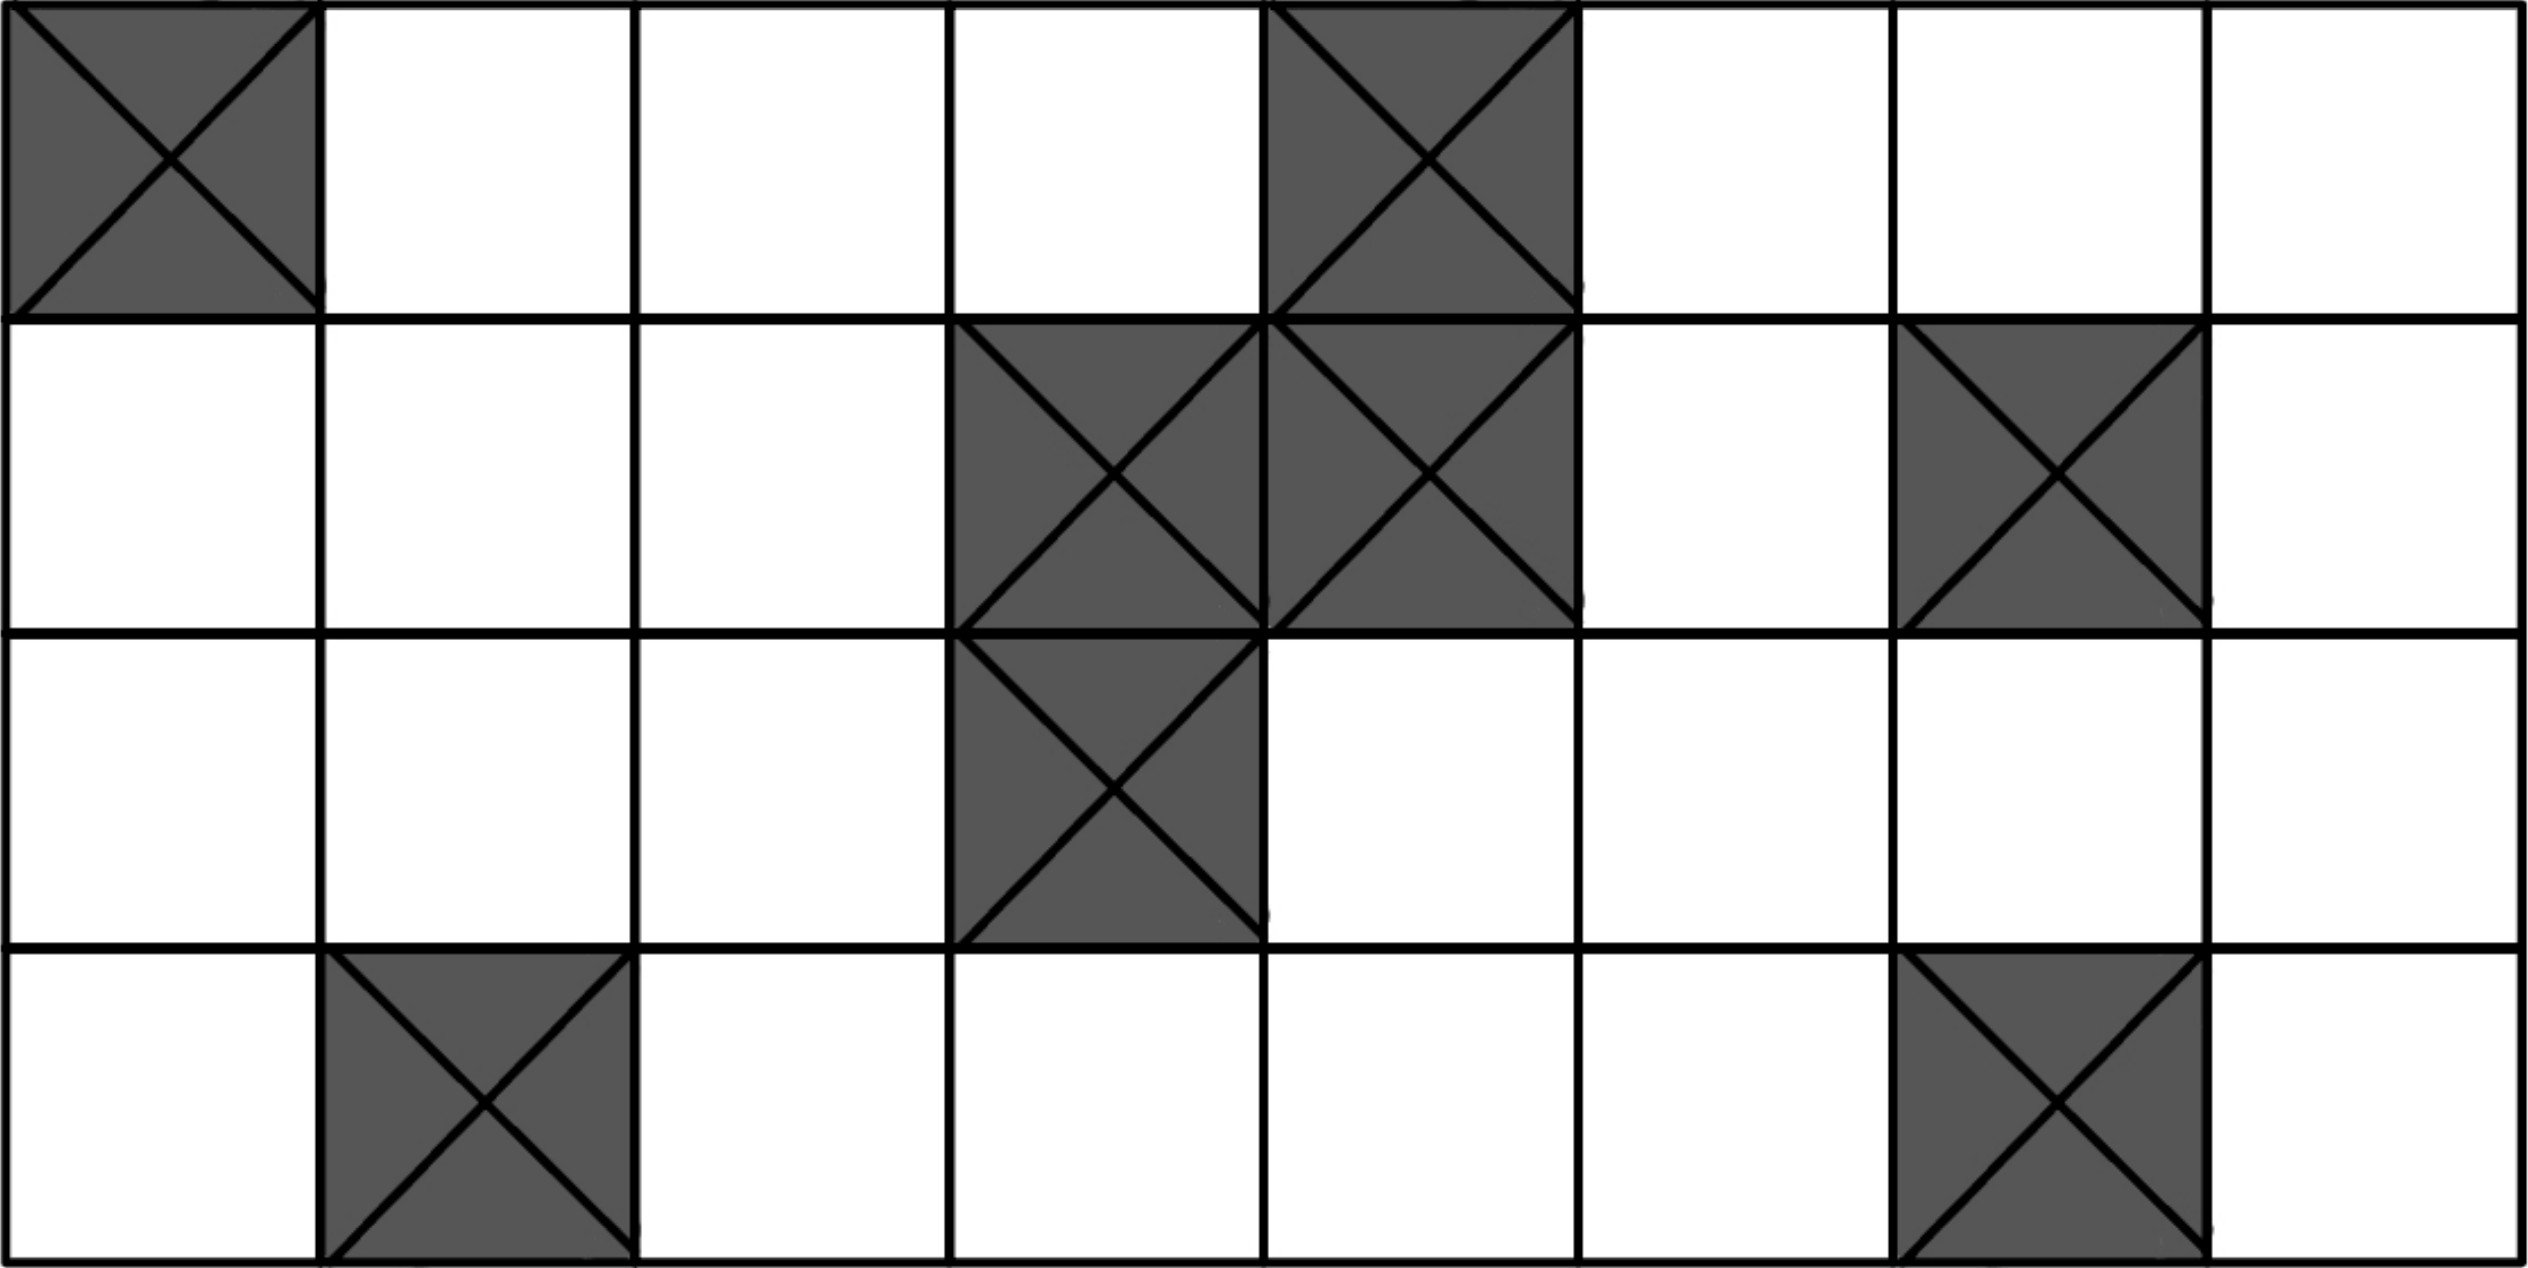
\includegraphics[scale=.2]{P5.png}  
    \]
\end{problem}
\begin{proof}

Here is the graph theory version of the problem, where vertices represent the squares and edges represent possible filings. Therefore, whether the board can be tiled is equivalent to saying whether the graph has a perfect matching.
\[\begin{tikzcd}
        % https://q.uiver.app/?q=WzAsMjQsWzAsMSwiXFxidWxsZXQiXSxbMCwyLCJcXGJ1bGxldCJdLFswLDMsIlxcYnVsbGV0Il0sWzIsMywiXFxidWxsZXQiXSxbMywzLCJcXGJ1bGxldCJdLFs0LDMsIlxcYnVsbGV0Il0sWzUsMywiXFxidWxsZXQiXSxbNSwyLCJcXGJ1bGxldCJdLFs1LDEsIlxcYnVsbGV0Il0sWzUsMCwiXFxidWxsZXQiXSxbMywwLCJcXGJ1bGxldCJdLFsxLDAsIlxcYnVsbGV0Il0sWzIsMCwiXFxidWxsZXQiXSxbNywzLCJcXGJ1bGxldCJdLFs3LDIsIlxcYnVsbGV0Il0sWzYsMiwiXFxidWxsZXQiXSxbNywxLCJcXGJ1bGxldCJdLFs2LDAsIlxcYnVsbGV0Il0sWzcsMCwiXFxidWxsZXQiXSxbNCwyLCJcXGJ1bGxldCJdLFsyLDEsIlxcYnVsbGV0Il0sWzIsMiwiXFxidWxsZXQiXSxbMSwyLCJcXGJ1bGxldCJdLFsxLDEsIlxcYnVsbGV0Il0sWzAsMjMsIiIsMCx7InN0eWxlIjp7ImhlYWQiOnsibmFtZSI6Im5vbmUifX19XSxbMjMsMjAsIiIsMCx7InN0eWxlIjp7ImhlYWQiOnsibmFtZSI6Im5vbmUifX19XSxbMSwyMiwiIiwwLHsic3R5bGUiOnsiaGVhZCI6eyJuYW1lIjoibm9uZSJ9fX1dLFsyMiwyMSwiIiwwLHsic3R5bGUiOnsiaGVhZCI6eyJuYW1lIjoibm9uZSJ9fX1dLFszLDQsIiIsMCx7InN0eWxlIjp7ImhlYWQiOnsibmFtZSI6Im5vbmUifX19XSxbNSw2LCIiLDAseyJzdHlsZSI6eyJoZWFkIjp7Im5hbWUiOiJub25lIn19fV0sWzE5LDcsIiIsMCx7InN0eWxlIjp7ImhlYWQiOnsibmFtZSI6Im5vbmUifX19XSxbMTEsMTIsIiIsMCx7InN0eWxlIjp7ImhlYWQiOnsibmFtZSI6Im5vbmUifX19XSxbMTIsMTAsIiIsMCx7InN0eWxlIjp7ImhlYWQiOnsibmFtZSI6Im5vbmUifX19XSxbOSwxNywiIiwwLHsic3R5bGUiOnsiaGVhZCI6eyJuYW1lIjoibm9uZSJ9fX1dLFsxNSwxNCwiIiwwLHsic3R5bGUiOnsiaGVhZCI6eyJuYW1lIjoibm9uZSJ9fX1dLFsyLDEsIiIsMCx7InN0eWxlIjp7ImhlYWQiOnsibmFtZSI6Im5vbmUifX19XSxbMSwwLCIiLDAseyJzdHlsZSI6eyJoZWFkIjp7Im5hbWUiOiJub25lIn19fV0sWzIyLDIzLCIiLDEseyJzdHlsZSI6eyJoZWFkIjp7Im5hbWUiOiJub25lIn19fV0sWzIzLDExLCIiLDEseyJzdHlsZSI6eyJoZWFkIjp7Im5hbWUiOiJub25lIn19fV0sWzIxLDIwLCIiLDEseyJzdHlsZSI6eyJoZWFkIjp7Im5hbWUiOiJub25lIn19fV0sWzIwLDEyLCIiLDEseyJzdHlsZSI6eyJoZWFkIjp7Im5hbWUiOiJub25lIn19fV0sWzMsMjEsIiIsMSx7InN0eWxlIjp7ImhlYWQiOnsibmFtZSI6Im5vbmUifX19XSxbNSwxOSwiIiwwLHsic3R5bGUiOnsiaGVhZCI6eyJuYW1lIjoibm9uZSJ9fX1dLFs2LDcsIiIsMSx7InN0eWxlIjp7ImhlYWQiOnsibmFtZSI6Im5vbmUifX19XSxbNyw4LCIiLDEseyJzdHlsZSI6eyJoZWFkIjp7Im5hbWUiOiJub25lIn19fV0sWzgsOSwiIiwxLHsic3R5bGUiOnsiaGVhZCI6eyJuYW1lIjoibm9uZSJ9fX1dLFsxNCwxNiwiIiwwLHsic3R5bGUiOnsiaGVhZCI6eyJuYW1lIjoibm9uZSJ9fX1dLFsxNiwxOCwiIiwwLHsic3R5bGUiOnsiaGVhZCI6eyJuYW1lIjoibm9uZSJ9fX1dLFsxMywxNCwiIiwwLHsic3R5bGUiOnsiaGVhZCI6eyJuYW1lIjoibm9uZSJ9fX1dLFsxNywxOCwiIiwxLHsic3R5bGUiOnsiaGVhZCI6eyJuYW1lIjoibm9uZSJ9fX1dLFs3LDE1LCIiLDEseyJzdHlsZSI6eyJoZWFkIjp7Im5hbWUiOiJub25lIn19fV0sWzQsNSwiIiwwLHsic3R5bGUiOnsiaGVhZCI6eyJuYW1lIjoibm9uZSJ9fX1dXQ==
	& \bullet & \bullet & \bullet && \bullet & \bullet & \bullet \\
	\bullet & \bullet & \bullet &&& \bullet && \bullet \\
	\bullet & \bullet & \bullet && \bullet & \bullet & \bullet & \bullet \\
	\bullet && \bullet & \bullet & \bullet & \bullet && \bullet
	\arrow[no head, from=2-1, to=2-2]
	\arrow[no head, from=2-2, to=2-3]
	\arrow[no head, from=3-1, to=3-2]
	\arrow[no head, from=3-2, to=3-3]
	\arrow[no head, from=4-3, to=4-4]
	\arrow[no head, from=4-5, to=4-6]
	\arrow[no head, from=3-5, to=3-6]
	\arrow[no head, from=1-2, to=1-3]
	\arrow[no head, from=1-3, to=1-4]
	\arrow[no head, from=1-6, to=1-7]
	\arrow[no head, from=3-7, to=3-8]
	\arrow[no head, from=4-1, to=3-1]
	\arrow[no head, from=3-1, to=2-1]
	\arrow[no head, from=3-2, to=2-2]
	\arrow[no head, from=2-2, to=1-2]
	\arrow[no head, from=3-3, to=2-3]
	\arrow[no head, from=2-3, to=1-3]
	\arrow[no head, from=4-3, to=3-3]
	\arrow[no head, from=4-5, to=3-5]
	\arrow[no head, from=4-6, to=3-6]
	\arrow[no head, from=3-6, to=2-6]
	\arrow[no head, from=2-6, to=1-6]
	\arrow[no head, from=3-8, to=2-8]
	\arrow[no head, from=2-8, to=1-8]
	\arrow[no head, from=4-8, to=3-8]
	\arrow[no head, from=1-7, to=1-8]
	\arrow[no head, from=3-6, to=3-7]
	\arrow[no head, from=4-4, to=4-5]
\end{tikzcd}\]

To apply Hall's Theorem, let's color the vertices to show that it's bipartite graph (checkerboard pattern):

\[\begin{tikzcd}
    % https://q.uiver.app/?q=WzAsMjQsWzAsMSwiXFxidWxsZXQiXSxbMCwyLCJcXGJ1bGxldCIsWzAsNjAsNjAsMV1dLFswLDMsIlxcYnVsbGV0Il0sWzIsMywiXFxidWxsZXQiXSxbMywzLCJcXGJ1bGxldCIsWzAsNjAsNjAsMV1dLFs0LDMsIlxcYnVsbGV0Il0sWzUsMywiXFxidWxsZXQiLFswLDYwLDYwLDFdXSxbNSwyLCJcXGJ1bGxldCJdLFs1LDEsIlxcYnVsbGV0IixbMCw2MCw2MCwxXV0sWzUsMCwiXFxidWxsZXQiXSxbMywwLCJcXGJ1bGxldCJdLFsxLDAsIlxcYnVsbGV0Il0sWzIsMCwiXFxidWxsZXQiLFswLDYwLDYwLDFdXSxbNywzLCJcXGJ1bGxldCIsWzAsNjAsNjAsMV1dLFs3LDIsIlxcYnVsbGV0Il0sWzYsMiwiXFxidWxsZXQiLFswLDYwLDYwLDFdXSxbNywxLCJcXGJ1bGxldCIsWzAsNjAsNjAsMV1dLFs2LDAsIlxcYnVsbGV0IixbMCw2MCw2MCwxXV0sWzcsMCwiXFxidWxsZXQiXSxbNCwyLCJcXGJ1bGxldCIsWzAsNjAsNjAsMV1dLFsyLDEsIlxcYnVsbGV0Il0sWzIsMiwiXFxidWxsZXQiLFswLDYwLDYwLDFdXSxbMSwyLCJcXGJ1bGxldCJdLFsxLDEsIlxcYnVsbGV0IixbMCw2MCw2MCwxXV0sWzAsMjMsIiIsMCx7InN0eWxlIjp7ImhlYWQiOnsibmFtZSI6Im5vbmUifX19XSxbMjMsMjAsIiIsMCx7InN0eWxlIjp7ImhlYWQiOnsibmFtZSI6Im5vbmUifX19XSxbMSwyMiwiIiwwLHsic3R5bGUiOnsiaGVhZCI6eyJuYW1lIjoibm9uZSJ9fX1dLFsyMiwyMSwiIiwwLHsic3R5bGUiOnsiaGVhZCI6eyJuYW1lIjoibm9uZSJ9fX1dLFszLDQsIiIsMCx7InN0eWxlIjp7ImhlYWQiOnsibmFtZSI6Im5vbmUifX19XSxbNSw2LCIiLDAseyJzdHlsZSI6eyJoZWFkIjp7Im5hbWUiOiJub25lIn19fV0sWzE5LDcsIiIsMCx7InN0eWxlIjp7ImhlYWQiOnsibmFtZSI6Im5vbmUifX19XSxbMTEsMTIsIiIsMCx7InN0eWxlIjp7ImhlYWQiOnsibmFtZSI6Im5vbmUifX19XSxbMTIsMTAsIiIsMCx7InN0eWxlIjp7ImhlYWQiOnsibmFtZSI6Im5vbmUifX19XSxbOSwxNywiIiwwLHsic3R5bGUiOnsiaGVhZCI6eyJuYW1lIjoibm9uZSJ9fX1dLFsxNSwxNCwiIiwwLHsic3R5bGUiOnsiaGVhZCI6eyJuYW1lIjoibm9uZSJ9fX1dLFsyLDEsIiIsMCx7InN0eWxlIjp7ImhlYWQiOnsibmFtZSI6Im5vbmUifX19XSxbMSwwLCIiLDAseyJzdHlsZSI6eyJoZWFkIjp7Im5hbWUiOiJub25lIn19fV0sWzIyLDIzLCIiLDEseyJzdHlsZSI6eyJoZWFkIjp7Im5hbWUiOiJub25lIn19fV0sWzIzLDExLCIiLDEseyJzdHlsZSI6eyJoZWFkIjp7Im5hbWUiOiJub25lIn19fV0sWzIxLDIwLCIiLDEseyJzdHlsZSI6eyJoZWFkIjp7Im5hbWUiOiJub25lIn19fV0sWzIwLDEyLCIiLDEseyJzdHlsZSI6eyJoZWFkIjp7Im5hbWUiOiJub25lIn19fV0sWzMsMjEsIiIsMSx7InN0eWxlIjp7ImhlYWQiOnsibmFtZSI6Im5vbmUifX19XSxbNSwxOSwiIiwwLHsic3R5bGUiOnsiaGVhZCI6eyJuYW1lIjoibm9uZSJ9fX1dLFs2LDcsIiIsMSx7InN0eWxlIjp7ImhlYWQiOnsibmFtZSI6Im5vbmUifX19XSxbNyw4LCIiLDEseyJzdHlsZSI6eyJoZWFkIjp7Im5hbWUiOiJub25lIn19fV0sWzgsOSwiIiwxLHsic3R5bGUiOnsiaGVhZCI6eyJuYW1lIjoibm9uZSJ9fX1dLFsxNCwxNiwiIiwwLHsic3R5bGUiOnsiaGVhZCI6eyJuYW1lIjoibm9uZSJ9fX1dLFsxNiwxOCwiIiwwLHsic3R5bGUiOnsiaGVhZCI6eyJuYW1lIjoibm9uZSJ9fX1dLFsxMywxNCwiIiwwLHsic3R5bGUiOnsiaGVhZCI6eyJuYW1lIjoibm9uZSJ9fX1dLFsxNywxOCwiIiwxLHsic3R5bGUiOnsiaGVhZCI6eyJuYW1lIjoibm9uZSJ9fX1dLFs3LDE1LCIiLDEseyJzdHlsZSI6eyJoZWFkIjp7Im5hbWUiOiJub25lIn19fV0sWzQsNSwiIiwwLHsic3R5bGUiOnsiaGVhZCI6eyJuYW1lIjoibm9uZSJ9fX1dXQ==
	& \bullet & \textcolor{rgb,255:red,214;green,92;blue,92}{\bullet} & \bullet && \bullet & \textcolor{rgb,255:red,214;green,92;blue,92}{\bullet} & \bullet \\
	\bullet & \textcolor{rgb,255:red,214;green,92;blue,92}{\bullet} & \bullet &&& \textcolor{rgb,255:red,214;green,92;blue,92}{\bullet} && \textcolor{rgb,255:red,214;green,92;blue,92}{\bullet} \\
	\textcolor{rgb,255:red,214;green,92;blue,92}{\bullet} & \bullet & \textcolor{rgb,255:red,214;green,92;blue,92}{\bullet} && \textcolor{rgb,255:red,214;green,92;blue,92}{\bullet} & \bullet & \textcolor{rgb,255:red,214;green,92;blue,92}{\bullet} & \bullet \\
	\bullet && \bullet & \textcolor{rgb,255:red,214;green,92;blue,92}{\bullet} & \bullet & \textcolor{rgb,255:red,214;green,92;blue,92}{\bullet} && \textcolor{rgb,255:red,214;green,92;blue,92}{\bullet}
	\arrow[no head, from=2-1, to=2-2]
	\arrow[no head, from=2-2, to=2-3]
	\arrow[no head, from=3-1, to=3-2]
	\arrow[no head, from=3-2, to=3-3]
	\arrow[no head, from=4-3, to=4-4]
	\arrow[no head, from=4-5, to=4-6]
	\arrow[no head, from=3-5, to=3-6]
	\arrow[no head, from=1-2, to=1-3]
	\arrow[no head, from=1-3, to=1-4]
	\arrow[no head, from=1-6, to=1-7]
	\arrow[no head, from=3-7, to=3-8]
	\arrow[no head, from=4-1, to=3-1]
	\arrow[no head, from=3-1, to=2-1]
	\arrow[no head, from=3-2, to=2-2]
	\arrow[no head, from=2-2, to=1-2]
	\arrow[no head, from=3-3, to=2-3]
	\arrow[no head, from=2-3, to=1-3]
	\arrow[no head, from=4-3, to=3-3]
	\arrow[no head, from=4-5, to=3-5]
	\arrow[no head, from=4-6, to=3-6]
	\arrow[no head, from=3-6, to=2-6]
	\arrow[no head, from=2-6, to=1-6]
	\arrow[no head, from=3-8, to=2-8]
	\arrow[no head, from=2-8, to=1-8]
	\arrow[no head, from=4-8, to=3-8]
	\arrow[no head, from=1-7, to=1-8]
	\arrow[no head, from=3-6, to=3-7]
	\arrow[no head, from=4-4, to=4-5]
\end{tikzcd}\]

Recall Hall's Theorem says a bipartite graph \(G = (X \sqcup Y, E)\) has matching saturating \(X\) iff \((\forall S \subset X)(|S| \leq |N(S)|)\). Therefore, if \((\exists S \subset X)(|S| > |N(S)|)\) we know a perfect matching is not possible, and we can see the set \(S = {s_1,s_2,s_3,s_4}\) (shown bellow) has only 3 neighbors, so \((\exists S \subset X)(|S| > |N(S)|)\) and a perfect matching is not possible.

\[\begin{tikzcd}
    % https://q.uiver.app/?q=WzAsMjQsWzAsMSwic18yIl0sWzAsMiwiXFxidWxsZXQiLFswLDYwLDYwLDFdXSxbMCwzLCJzXzEiXSxbMiwzLCJcXGJ1bGxldCJdLFszLDMsIlxcYnVsbGV0IixbMCw2MCw2MCwxXV0sWzQsMywiXFxidWxsZXQiXSxbNSwzLCJcXGJ1bGxldCIsWzAsNjAsNjAsMV1dLFs1LDIsIlxcYnVsbGV0Il0sWzUsMSwiXFxidWxsZXQiLFswLDYwLDYwLDFdXSxbNSwwLCJcXGJ1bGxldCJdLFszLDAsInNfNCJdLFsxLDAsInNfMyJdLFsyLDAsIlxcYnVsbGV0IixbMCw2MCw2MCwxXV0sWzcsMywiXFxidWxsZXQiLFswLDYwLDYwLDFdXSxbNywyLCJcXGJ1bGxldCJdLFs2LDIsIlxcYnVsbGV0IixbMCw2MCw2MCwxXV0sWzcsMSwiXFxidWxsZXQiLFswLDYwLDYwLDFdXSxbNiwwLCJcXGJ1bGxldCIsWzAsNjAsNjAsMV1dLFs3LDAsIlxcYnVsbGV0Il0sWzQsMiwiXFxidWxsZXQiLFswLDYwLDYwLDFdXSxbMiwxLCJcXGJ1bGxldCJdLFsyLDIsIlxcYnVsbGV0IixbMCw2MCw2MCwxXV0sWzEsMiwiXFxidWxsZXQiXSxbMSwxLCJcXGJ1bGxldCIsWzAsNjAsNjAsMV1dLFswLDIzLCIiLDAseyJzdHlsZSI6eyJoZWFkIjp7Im5hbWUiOiJub25lIn19fV0sWzIzLDIwLCIiLDAseyJzdHlsZSI6eyJoZWFkIjp7Im5hbWUiOiJub25lIn19fV0sWzEsMjIsIiIsMCx7InN0eWxlIjp7ImhlYWQiOnsibmFtZSI6Im5vbmUifX19XSxbMjIsMjEsIiIsMCx7InN0eWxlIjp7ImhlYWQiOnsibmFtZSI6Im5vbmUifX19XSxbMyw0LCIiLDAseyJzdHlsZSI6eyJoZWFkIjp7Im5hbWUiOiJub25lIn19fV0sWzUsNiwiIiwwLHsic3R5bGUiOnsiaGVhZCI6eyJuYW1lIjoibm9uZSJ9fX1dLFsxOSw3LCIiLDAseyJzdHlsZSI6eyJoZWFkIjp7Im5hbWUiOiJub25lIn19fV0sWzExLDEyLCIiLDAseyJzdHlsZSI6eyJoZWFkIjp7Im5hbWUiOiJub25lIn19fV0sWzksMTcsIiIsMCx7InN0eWxlIjp7ImhlYWQiOnsibmFtZSI6Im5vbmUifX19XSxbMTUsMTQsIiIsMCx7InN0eWxlIjp7ImhlYWQiOnsibmFtZSI6Im5vbmUifX19XSxbMiwxLCIiLDAseyJzdHlsZSI6eyJoZWFkIjp7Im5hbWUiOiJub25lIn19fV0sWzEsMCwiIiwwLHsic3R5bGUiOnsiaGVhZCI6eyJuYW1lIjoibm9uZSJ9fX1dLFsyMiwyMywiIiwxLHsic3R5bGUiOnsiaGVhZCI6eyJuYW1lIjoibm9uZSJ9fX1dLFsyMywxMSwiIiwxLHsic3R5bGUiOnsiaGVhZCI6eyJuYW1lIjoibm9uZSJ9fX1dLFsyMSwyMCwiIiwxLHsic3R5bGUiOnsiaGVhZCI6eyJuYW1lIjoibm9uZSJ9fX1dLFsyMCwxMiwiIiwxLHsic3R5bGUiOnsiaGVhZCI6eyJuYW1lIjoibm9uZSJ9fX1dLFszLDIxLCIiLDEseyJzdHlsZSI6eyJoZWFkIjp7Im5hbWUiOiJub25lIn19fV0sWzUsMTksIiIsMCx7InN0eWxlIjp7ImhlYWQiOnsibmFtZSI6Im5vbmUifX19XSxbNiw3LCIiLDEseyJzdHlsZSI6eyJoZWFkIjp7Im5hbWUiOiJub25lIn19fV0sWzcsOCwiIiwxLHsic3R5bGUiOnsiaGVhZCI6eyJuYW1lIjoibm9uZSJ9fX1dLFs4LDksIiIsMSx7InN0eWxlIjp7ImhlYWQiOnsibmFtZSI6Im5vbmUifX19XSxbMTQsMTYsIiIsMCx7InN0eWxlIjp7ImhlYWQiOnsibmFtZSI6Im5vbmUifX19XSxbMTYsMTgsIiIsMCx7InN0eWxlIjp7ImhlYWQiOnsibmFtZSI6Im5vbmUifX19XSxbMTMsMTQsIiIsMCx7InN0eWxlIjp7ImhlYWQiOnsibmFtZSI6Im5vbmUifX19XSxbMTcsMTgsIiIsMSx7InN0eWxlIjp7ImhlYWQiOnsibmFtZSI6Im5vbmUifX19XSxbNywxNSwiIiwxLHsic3R5bGUiOnsiaGVhZCI6eyJuYW1lIjoibm9uZSJ9fX1dLFs0LDUsIiIsMCx7InN0eWxlIjp7ImhlYWQiOnsibmFtZSI6Im5vbmUifX19XSxbMTIsMTAsIiIsMCx7InN0eWxlIjp7ImhlYWQiOnsibmFtZSI6Im5vbmUifX19XV0=
	& {s_3} & \textcolor{rgb,255:red,214;green,92;blue,92}{\bullet} & {s_4} && \bullet & \textcolor{rgb,255:red,214;green,92;blue,92}{\bullet} & \bullet \\
	{s_2} & \textcolor{rgb,255:red,214;green,92;blue,92}{\bullet} & \bullet &&& \textcolor{rgb,255:red,214;green,92;blue,92}{\bullet} && \textcolor{rgb,255:red,214;green,92;blue,92}{\bullet} \\
	\textcolor{rgb,255:red,214;green,92;blue,92}{\bullet} & \bullet & \textcolor{rgb,255:red,214;green,92;blue,92}{\bullet} && \textcolor{rgb,255:red,214;green,92;blue,92}{\bullet} & \bullet & \textcolor{rgb,255:red,214;green,92;blue,92}{\bullet} & \bullet \\
	{s_1} && \bullet & \textcolor{rgb,255:red,214;green,92;blue,92}{\bullet} & \bullet & \textcolor{rgb,255:red,214;green,92;blue,92}{\bullet} && \textcolor{rgb,255:red,214;green,92;blue,92}{\bullet}
	\arrow[no head, from=2-1, to=2-2]
	\arrow[no head, from=2-2, to=2-3]
	\arrow[no head, from=3-1, to=3-2]
	\arrow[no head, from=3-2, to=3-3]
	\arrow[no head, from=4-3, to=4-4]
	\arrow[no head, from=4-5, to=4-6]
	\arrow[no head, from=3-5, to=3-6]
	\arrow[no head, from=1-2, to=1-3]
	\arrow[no head, from=1-6, to=1-7]
	\arrow[no head, from=3-7, to=3-8]
	\arrow[no head, from=4-1, to=3-1]
	\arrow[no head, from=3-1, to=2-1]
	\arrow[no head, from=3-2, to=2-2]
	\arrow[no head, from=2-2, to=1-2]
	\arrow[no head, from=3-3, to=2-3]
	\arrow[no head, from=2-3, to=1-3]
	\arrow[no head, from=4-3, to=3-3]
	\arrow[no head, from=4-5, to=3-5]
	\arrow[no head, from=4-6, to=3-6]
	\arrow[no head, from=3-6, to=2-6]
	\arrow[no head, from=2-6, to=1-6]
	\arrow[no head, from=3-8, to=2-8]
	\arrow[no head, from=2-8, to=1-8]
	\arrow[no head, from=4-8, to=3-8]
	\arrow[no head, from=1-7, to=1-8]
	\arrow[no head, from=3-6, to=3-7]
	\arrow[no head, from=4-4, to=4-5]
	\arrow[no head, from=1-3, to=1-4]
\end{tikzcd}\]
\end{proof}

\end{document}
